\section{Simulink Diagrams}\label{sec:simulink}
\subsection{Problem 2}
\begin{figure}[h]
	\centering
		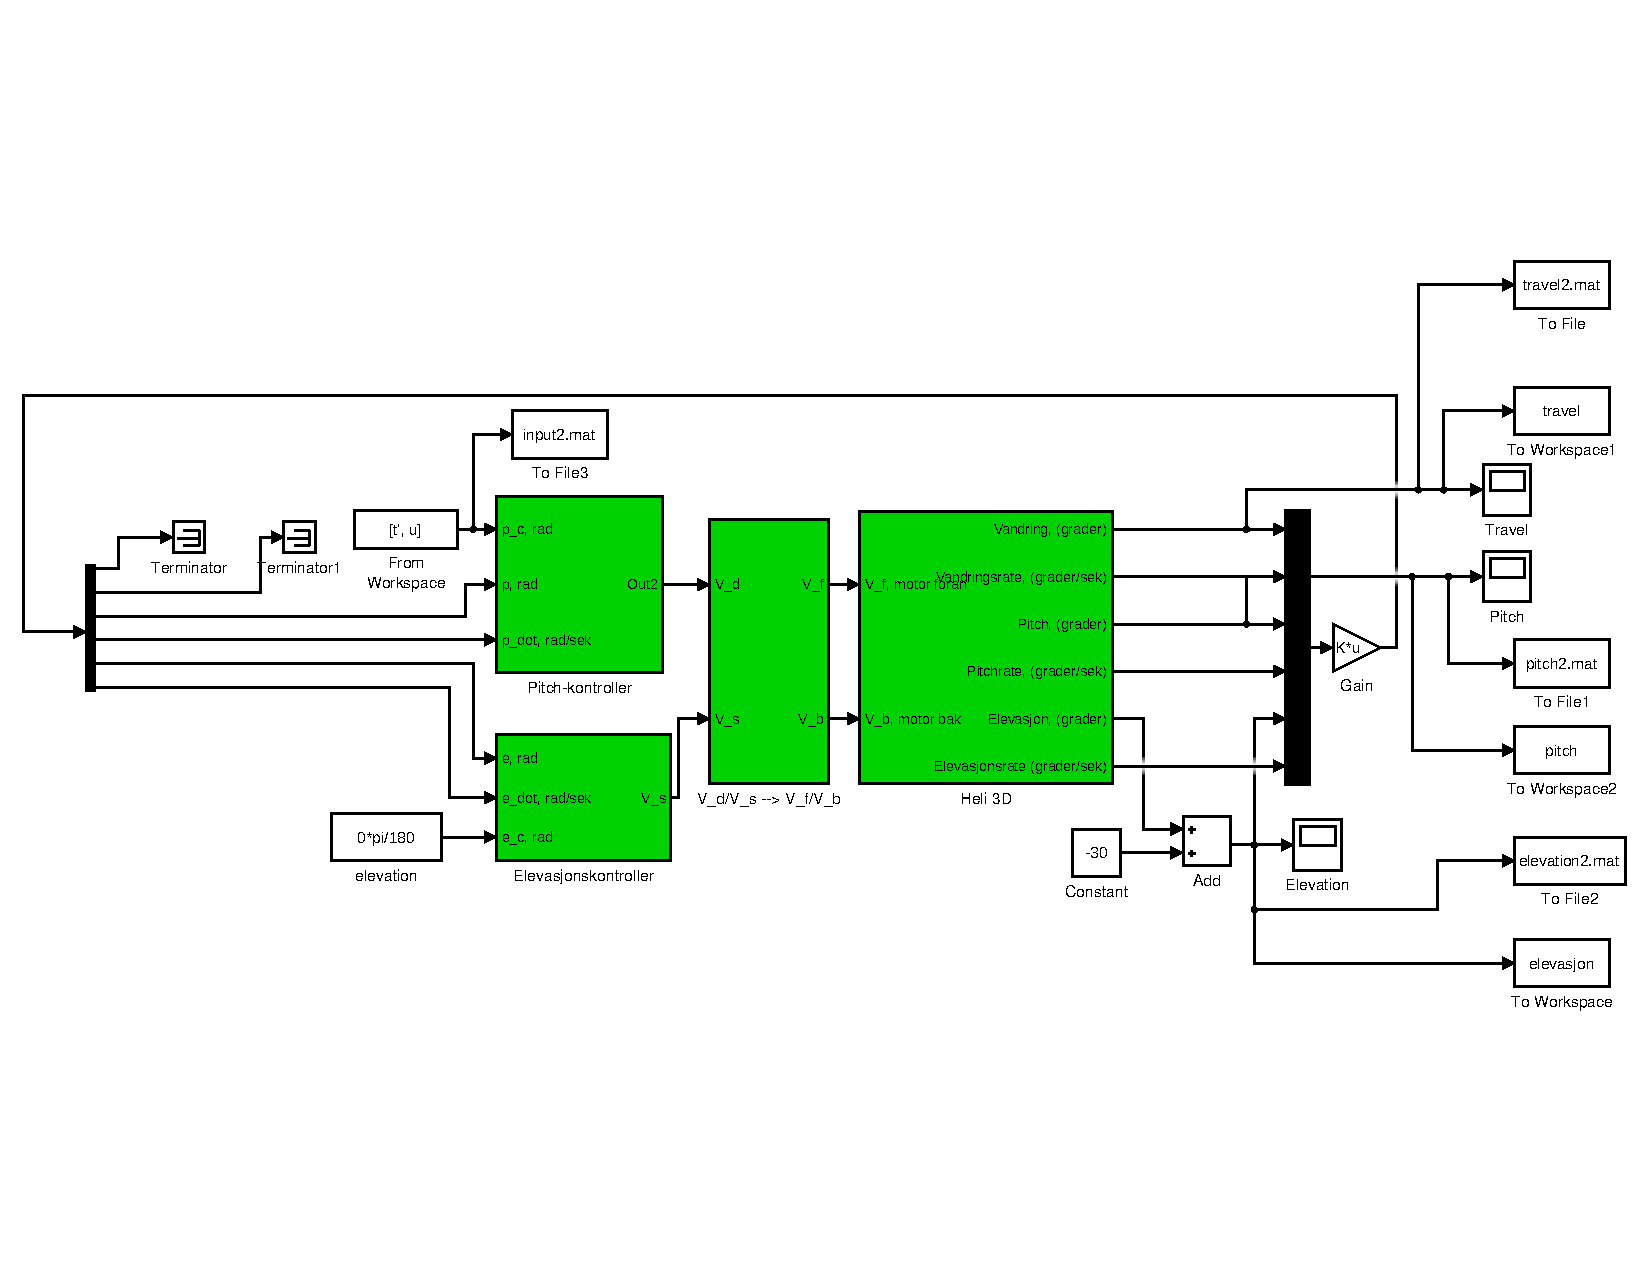
\includegraphics[trim=0 120 0 120,clip,width = \textwidth]{figures/problem2_simulink.pdf}
	\caption{Simulink diagram of problem 2.}
	\label{fig:problem2_simulink}
\end{figure}
\clearpage
\subsection{Problem 3}
\begin{figure}[h]
	\centering
	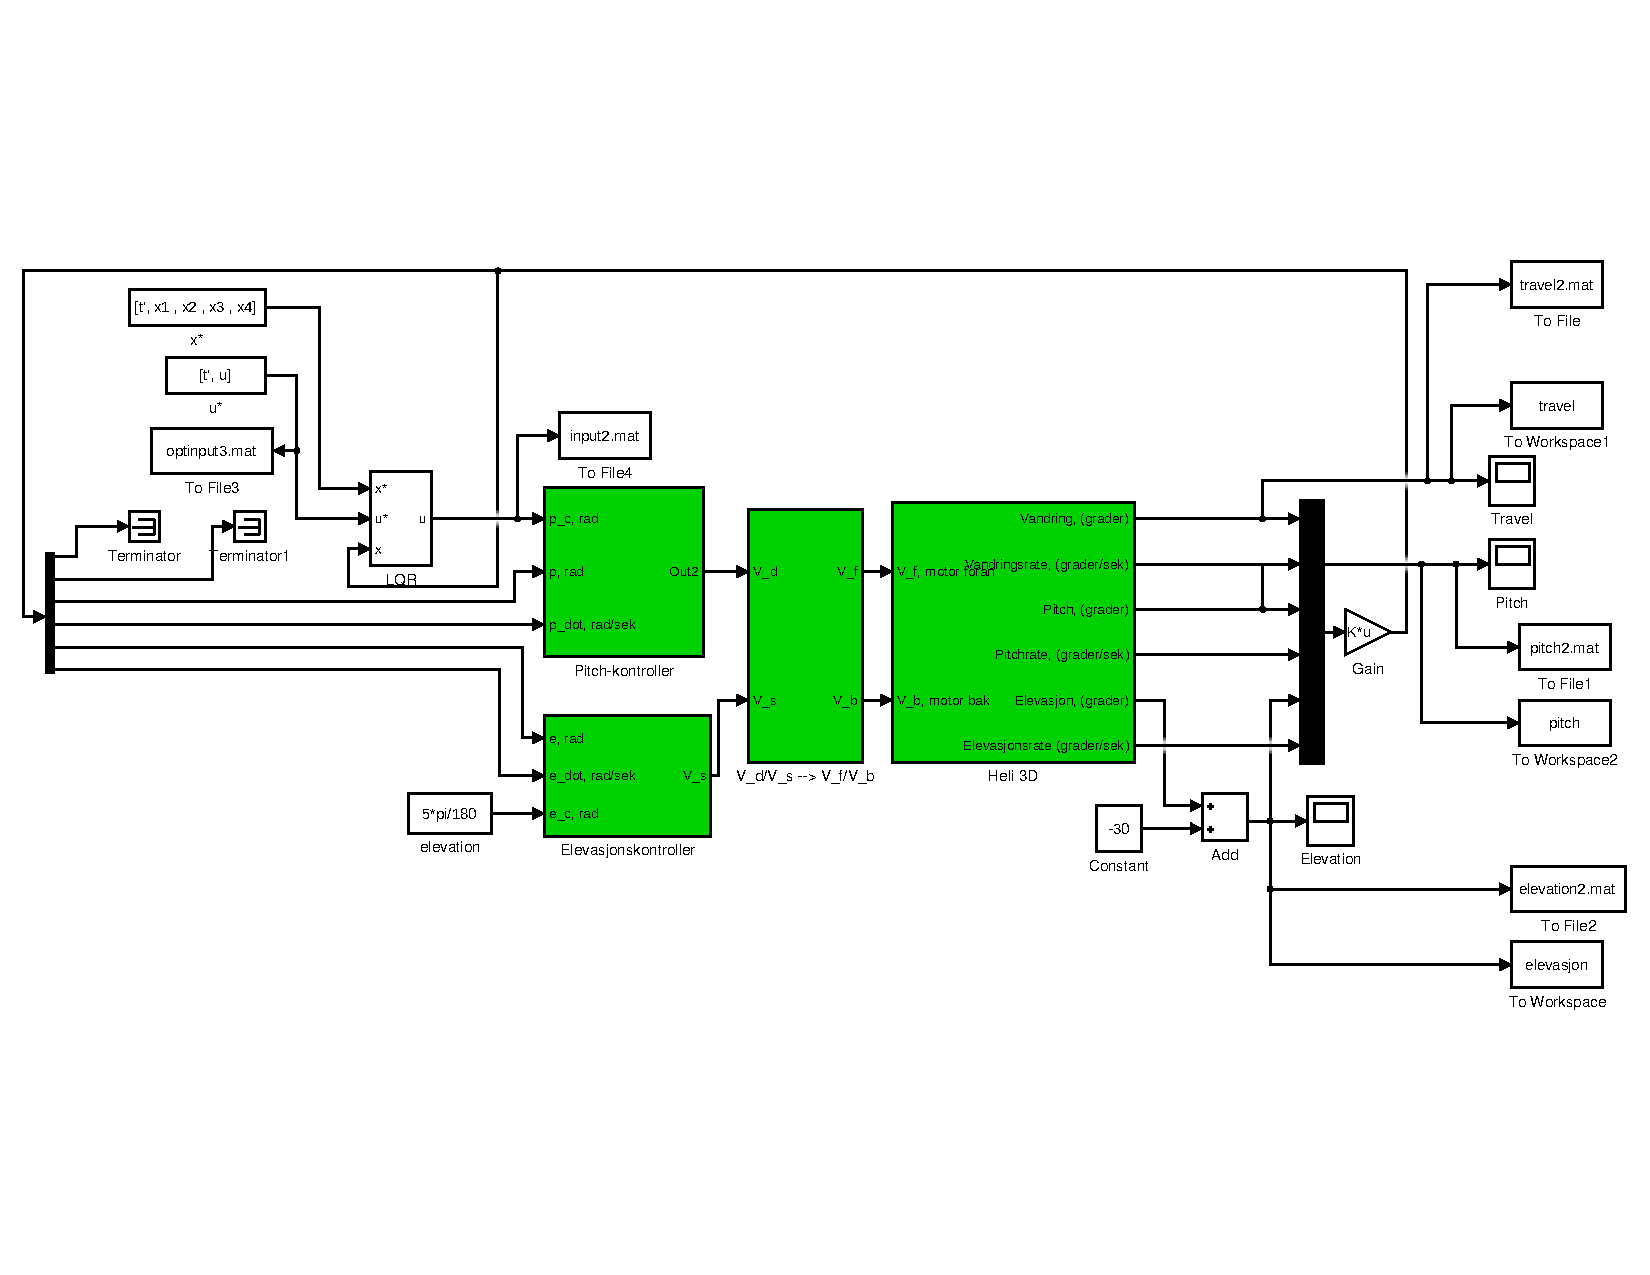
\includegraphics[trim=0 120 0 120,clip,width = \textwidth]{figures/problem3_simulink.pdf}
	\caption{Simulink diagram of problem 3.}
	\label{fig:problem3_simulink}
\end{figure}

\begin{figure}[h]
	\centering
	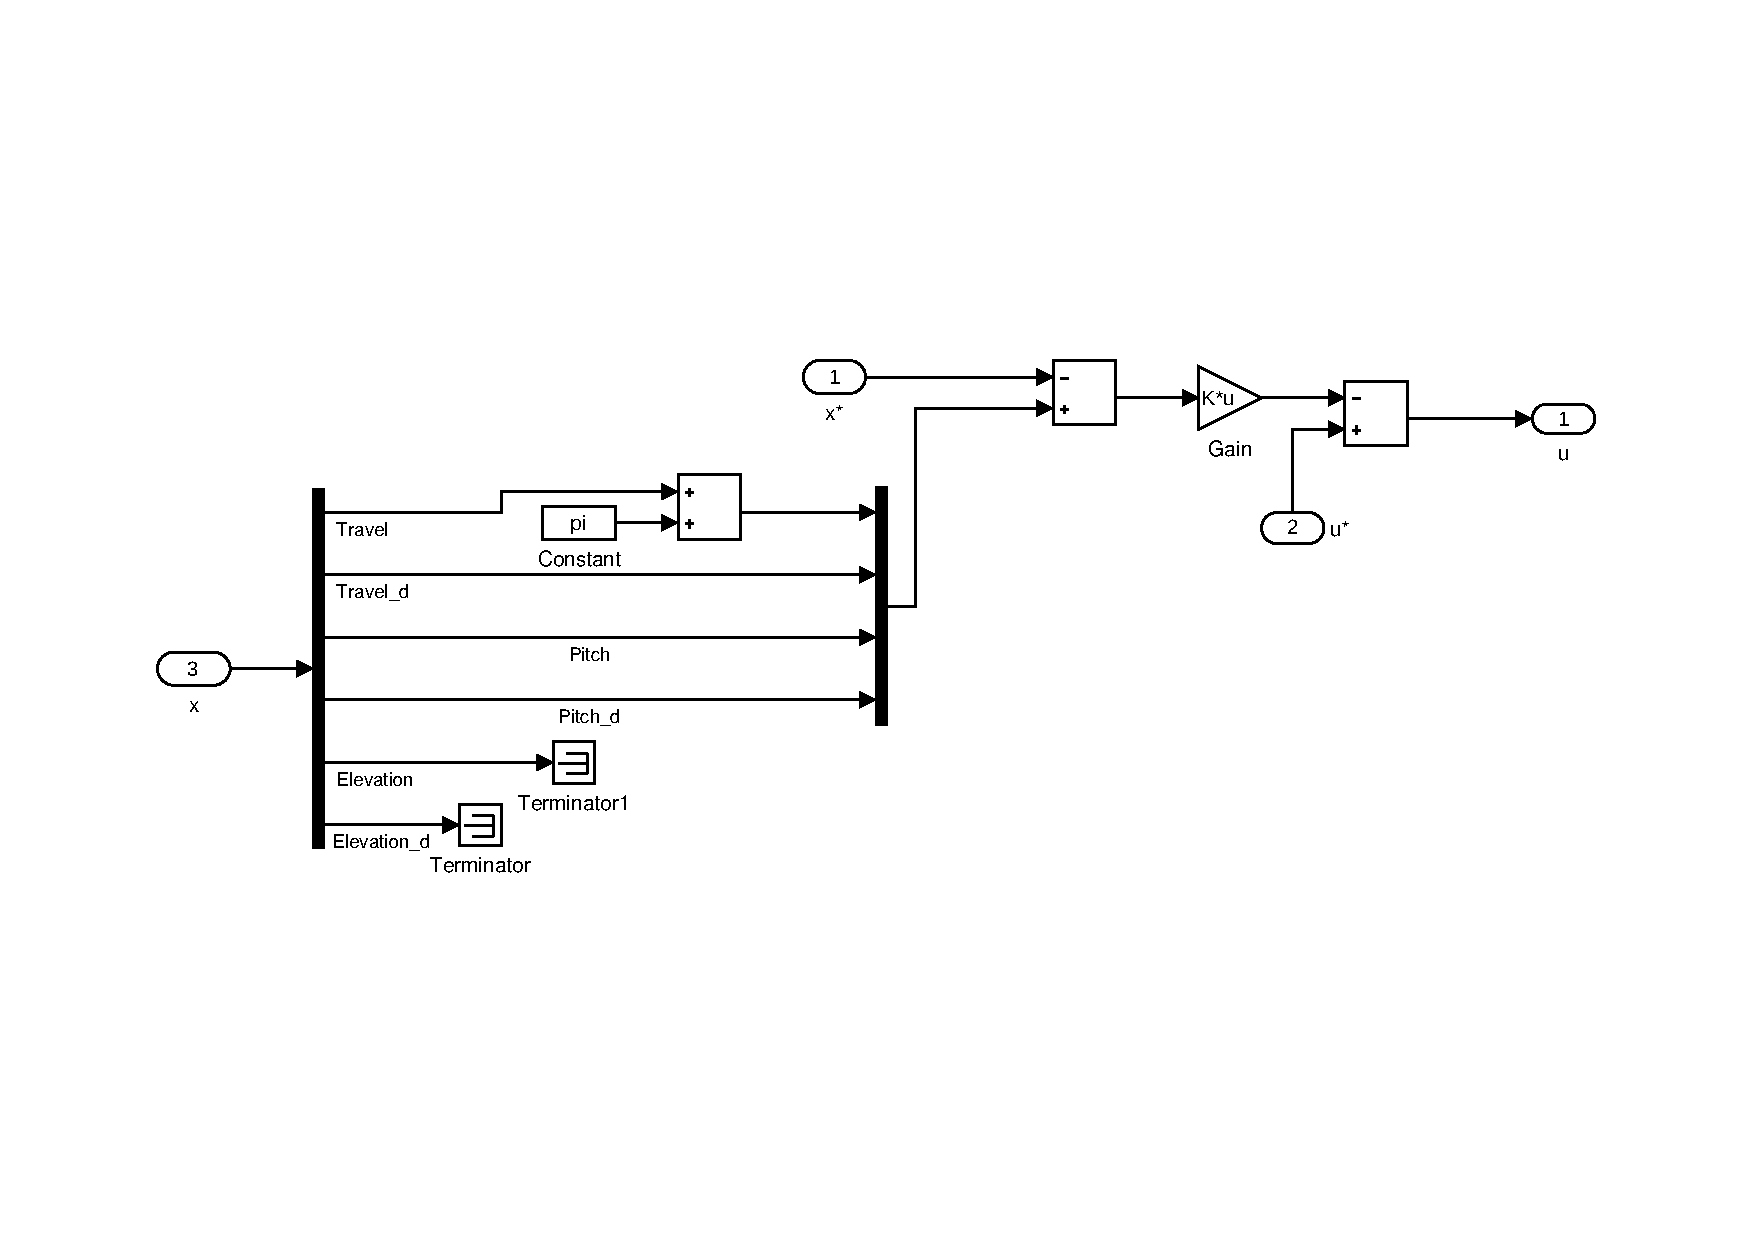
\includegraphics[trim=0 150 0 150,clip,width = \textwidth]{figures/problem3_lqr_simulink.pdf}
	\caption{Simulink diagram of LQR subsystem of problem 3.}
	\label{fig:problem3_lqr_simulink}
\end{figure}
\clearpage
\subsection{Problem 4}
\begin{figure}[h]
	\centering
	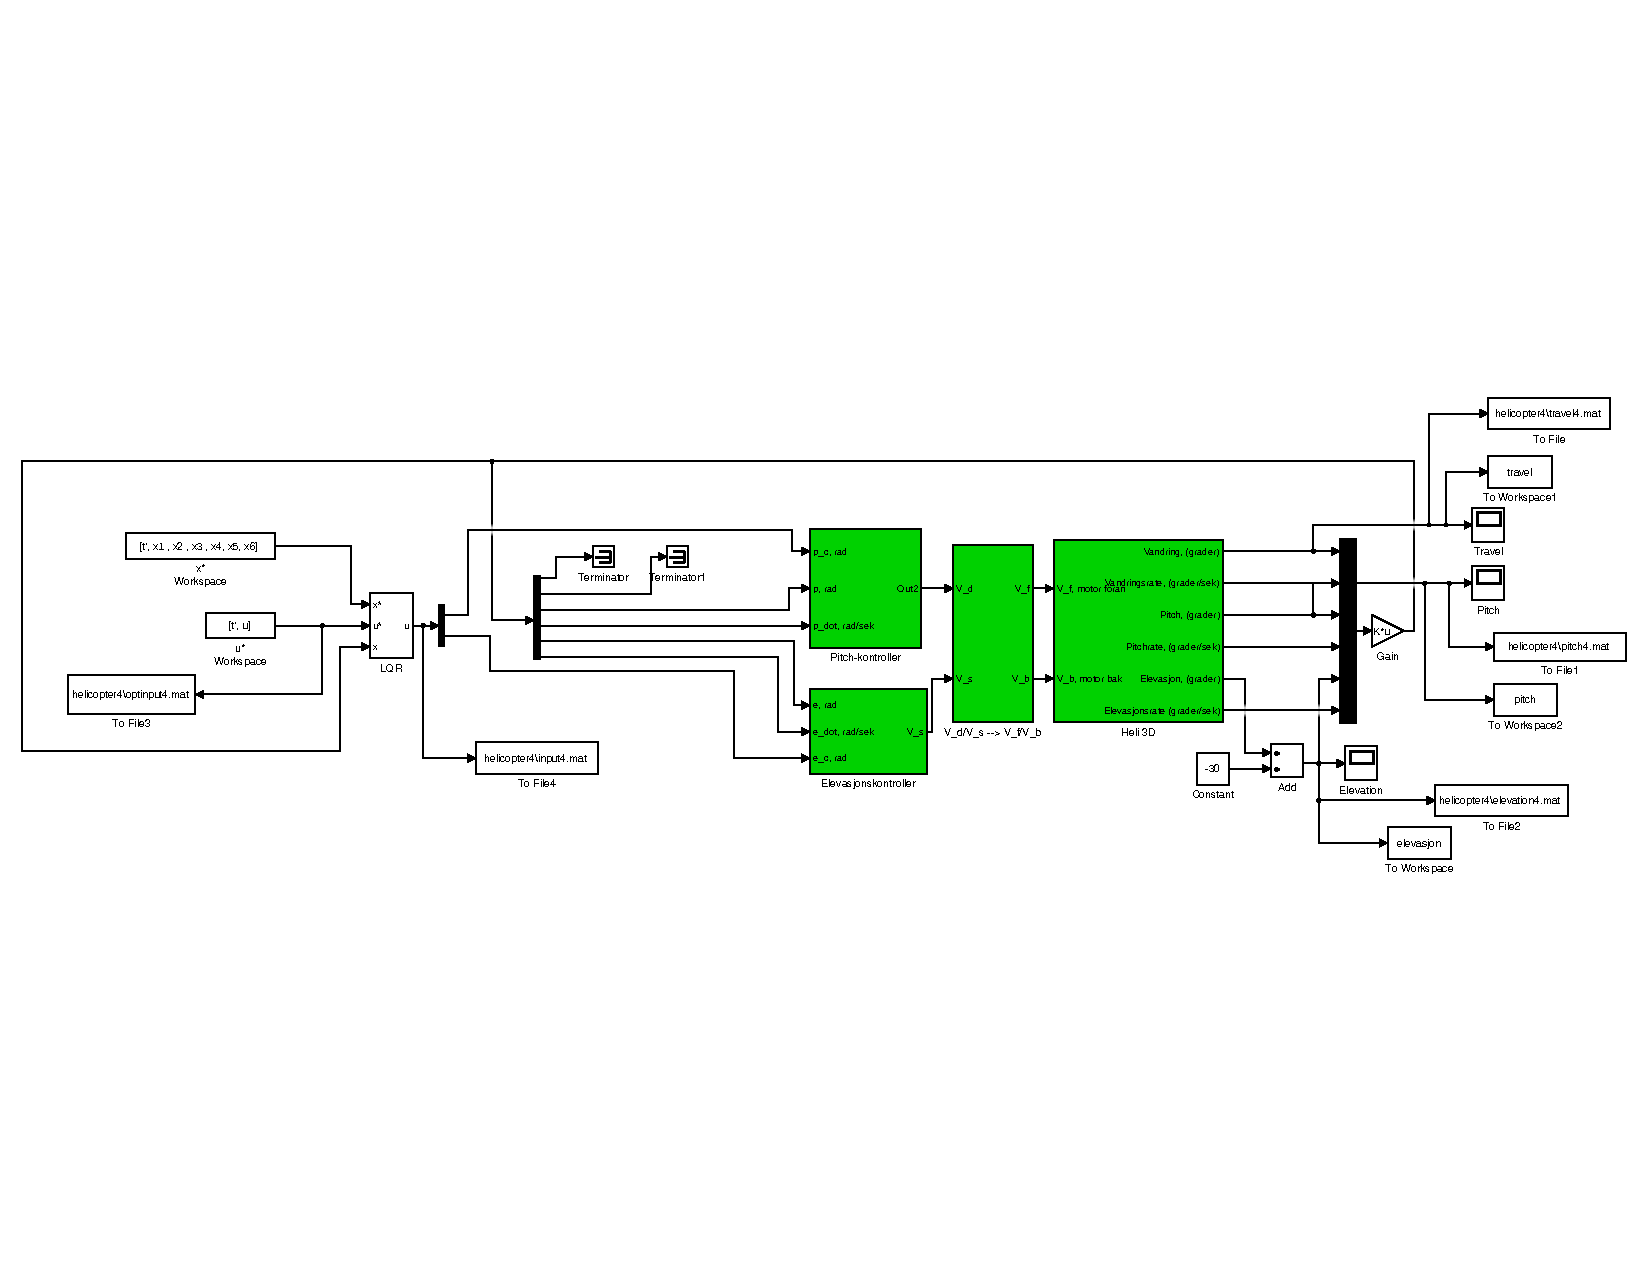
\includegraphics[trim=0 190 0 190,clip,width = \textwidth]{figures/problem4_simulink.pdf}
	\caption{Simulink diagram of problem 4.}
	\label{fig:problem4_simulink}
\end{figure}

\begin{figure}[h]
	\centering
	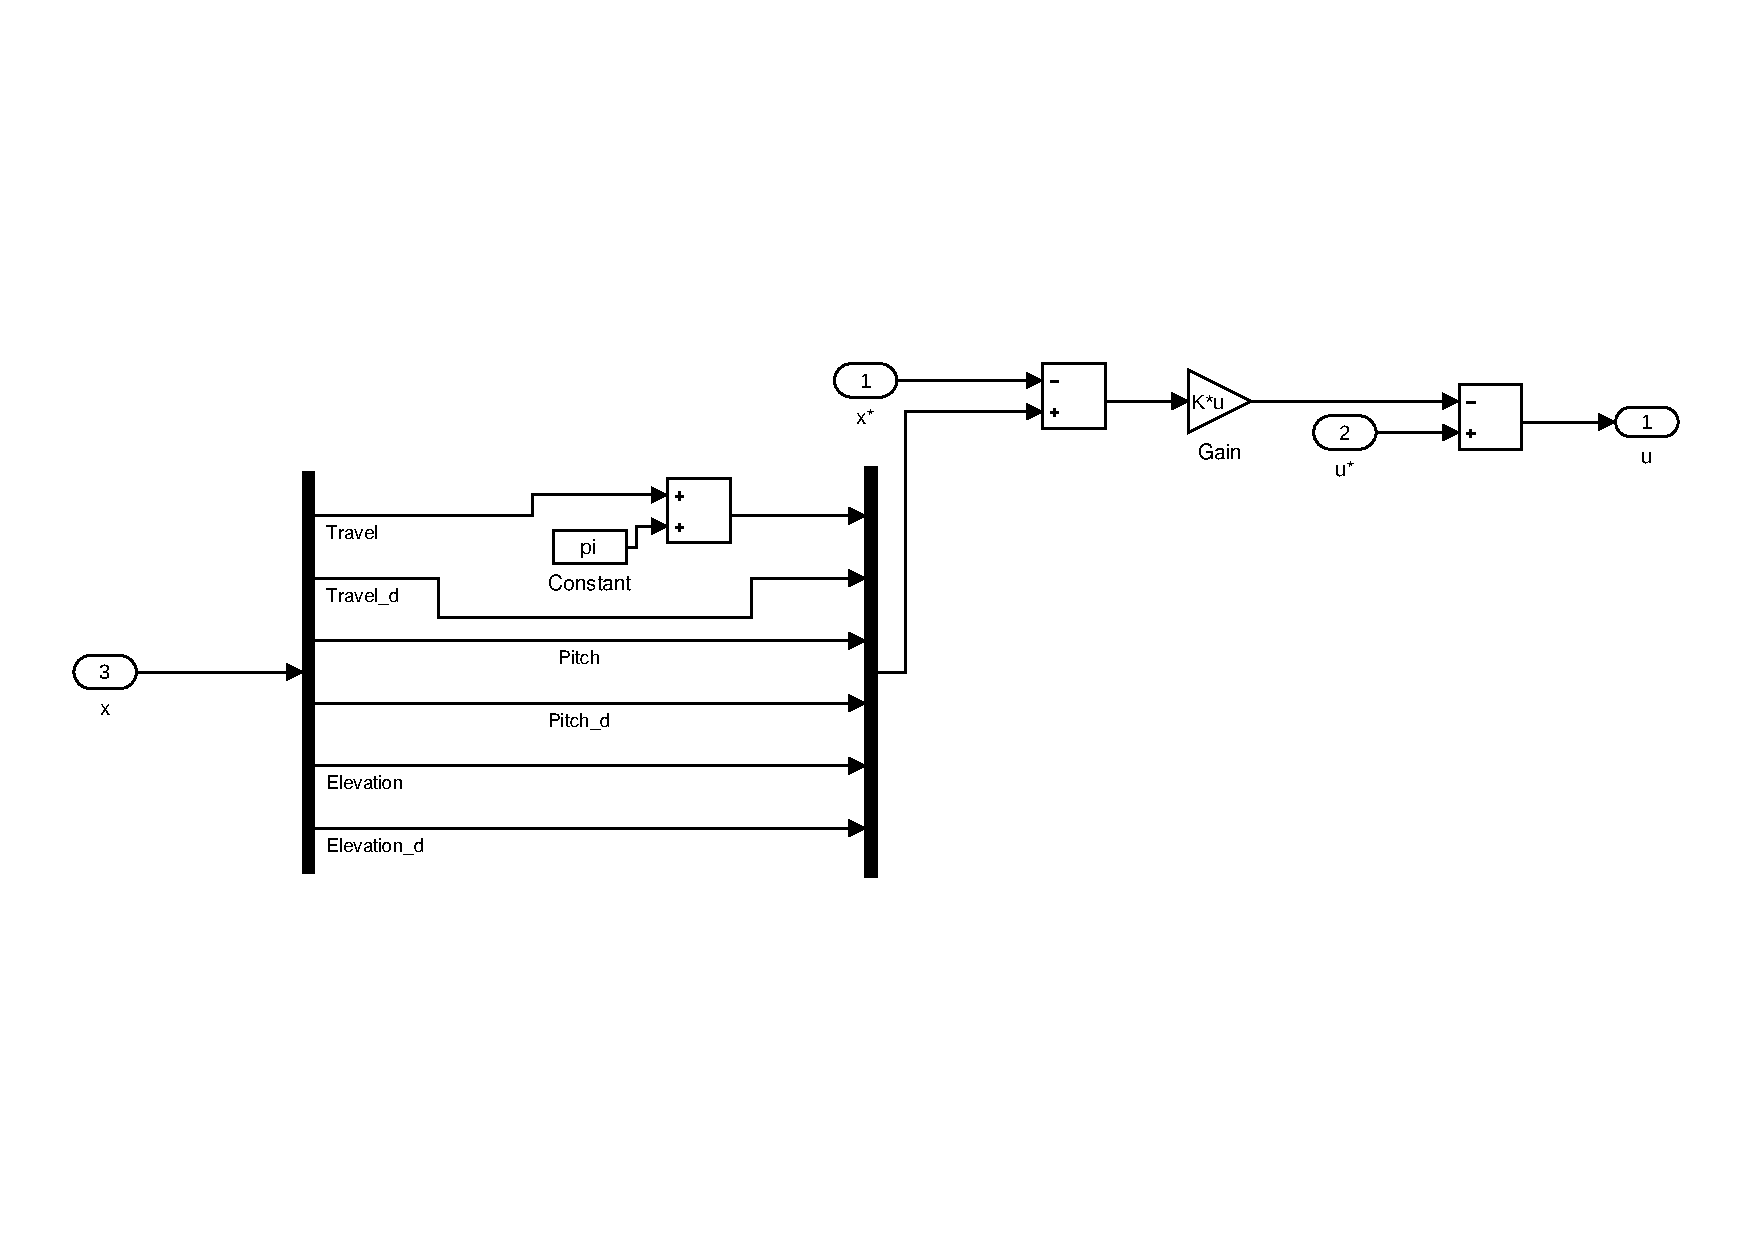
\includegraphics[trim=0 150 0 150,clip,width = \textwidth]{figures/problem4_lqr_simulink.pdf}
	\caption{Simulink diagram of LQR subsystem of problem 4.}
	\label{fig:problem4_lqr_simulink}
\end{figure}
